\documentclass[12pt]{article}

% Packages
\usepackage[utf8]{inputenc} % Allows input of UTF-8 characters
\usepackage[T1]{fontenc} % Output font encoding for international characters
\usepackage{geometry} % For setting margins
\usepackage{times} % Times New Roman font
\usepackage{graphicx} % For including images
\usepackage{amsmath} % Math environments and symbols
\usepackage{amsfonts} % mathbb
\usepackage{hyperref}
\usepackage{float}
\usepackage{caption}
\usepackage{subcaption}
\usepackage{enumitem}


\newcommand{\vct}[1]{\mathbf{#1}}
\newcommand{\mtx}[1]{\mathbf{#1}}

\geometry{margin=1in}
\setlength{\parskip}{0.5em}
\setlist[itemize]{itemsep=0pt, topsep=0pt}

\title{
  Physical Audio Modeling of Passive Rigid Bodies\\
  \large Real-time Interactive Audio Generation Using Linear Modal Analysis
}

\author{Karl Hiner\\khiner6@gatech.edu}
\date{\today}

\begin{document}

\maketitle

\section{Abstract}

An impact on the surface of a passive rigid body produces mechanical vibrations that propagate through the material.
As the excited object vibrates, its surface interacts with particles in the surrounding medium, producing longitudinal pressure waves that can be heard by a nearby listener.
The nature of the audio signal heard by such a listener is determined by the dynamics of these pressure waves, and these dynamics depend on many factors --- the material and geometry of the object, the excitation instrument and impact location, objects and boundaries in the environment, and even the geometry of the listener \cite{starch_perimetry_1908}.
Several highly general methods are available to accurately model the dynamics of acoustic radiation in the presence of complex geometries \cite{wang_wbss_2018} and dynamic, granular boundary conditions \cite{schneider_fdtd_2010}.
However, these methods are computationally intractable for settings such as video games and virtual realities, which require real-time execution on consumer hardware.
This work investigates computationally efficient methods for estimating the time-varying sound pressure level at a point in a 3D environment with passive rigid bodies radiating acoustic waves in response to impact forces on their surface.
By comparing results with a recently released large-scale dataset of real object impact sounds \cite{clarke_realimpact_2023}, we show that the well-known and efficient method of Linear Modal Analysis achieves qualitatively satisfactory results but often fails to accurately capture perceptually relevant vibrational modes using available material and geometry data.
Additionally, we provide an interactive 3D application for generating modal audio models from surface meshes and evaluating the excitation audio against real-world recordings.
While our quantitative evaluation is preliminary, we hope this study and accompanying application aid audio modeling researchers and interactive experience designers in developing efficient and physically accurate rigid body audio models.

\section{Introduction}

\subsection{Acoustic Radiation}

This work focuses on the dynamics of mechanical waves.
However, since our broad goal is to accurately model audio in interactive environements, an understanding of acoustic radiation is fundamental.
Acoustic wave propagation can be described by a scalar pressure field $P(\vct{x}, t)$, where $\vct{x}$ is a 3D position vector, and $\mathbf{v}(\vct{x}, t)$ is the vector velocity field, representing the velocity of the medium's particles as pressure waves propagate through it.
The key material parameters are the speed of sound $c_a$ and the medium's particle density $\rho$, which affects its acoustic impedance.

The governing equations of acoustic radiation can expressed as coupled first-order differential equations relating the temporal derivative of the pressure field to the spatial derivative of the velocity field:
\begin{align*}
\frac{\partial P}{\partial t} &= -\rho c_a^2 \nabla \cdot \mathbf{v},\\
\frac{\partial \mathbf{v}}{\partial t} &= -\frac{1}{\rho}\nabla P
\end{align*}
From these equations, the wave equation can be derived (as detailed in \textit{Schneider, 2010} \cite{schneider_fdtd_2010}):
$$\nabla^2P - \frac{1}{c_a^2}\frac{\partial^2 P}{\partial t^2} = 0$$
A solution particularly relevant for modeling sound wave dynamics is the harmonic plane wave, described by:
$$P(\vct{x},t) = P_0 e^{j(\omega t - \vct{k} \cdot \vct{x})},$$
where $P_0$ is the amplitude of the pressure wave, $\omega$ is the angular frequency, and $\vct{k}$ is the wave propagation vector.

Linearity only holds generally in \textit{small-signal acoustics}, when the amplitudes of the pressure waves are small enough that the dynamics do not significantly affect the properties of the propagating medium.
Throughout this work, we assume small-scale acoustic dynamics.
\footnote{This is a physical justification for the ubiquitous practice of modeling the combined sound pressure of multiple audio waves incident at a given point by simply summing them.}

\subsection{Linear Modal Analysis}

Linear Modal Analysis (LMA) is a computational technique used to model the vibrational dynamics of structures in response to external forces, and is based on solving the linear elastodynamic equation,
$$\mtx{M}\ddot{\vct{u}} + \mtx{C}\dot{\mtx{u}} + \mtx{K}\vct{u} = \vct{f},$$
where $\vct{u}(t)$ is the displacement vector of $N$ mesh nodes, $\mtx{M}, \mtx{C},$ and $\mtx{K}$ are the mass, damping, and stiffness matrices, and $\vct{f}(t)$ is the external force vector.

For this study, we adopt the common \textit{Rayleigh Damping} assumption that the damping of the system is fully characterized by a linear combination of its inertial and elastic effects.
Under this assumption, we express the damping matrix as
$$\mtx{C} = \alpha \mtx{M} + \beta \mtx{K},$$
where \(\alpha\) and \(\beta\) are scalars.

LMA assumes solutions to the dynamic problem have the form $\vct{u}(t) = \mtx{\Phi}\vct{q}(t),$ where $\mtx{\Phi}$ is the modal matrix with $\mtx{\Phi}_i \in \mathbb{R}^{3N}$ representing the $i$th "mode shape", and $\vct{q}(t)$ the corresponding modal amplitudes, assumed to be exponentially-decaying sinusoids.
Substituting yields the eigenvalue problem
\begin{equation}\label{eq:EigenvalueProblem}
  \mtx{K}\mtx{\Phi} = \mtx{\Lambda} \mtx{M}\mtx{\Phi},
\end{equation}
where $\mtx{\Lambda}$ is the diagonal matrix of eigenvalues.

This decomposition facilitates decoupling the global motion into individual modal contributions, which can be computed (and cached) independently and combined by linear superposition.
The system of decoupled ordinary differential equations can be written as
$$\ddot{q}_i + 2\xi_i \omega_i \dot{q}_i + \omega_i^2 q_i = \frac{Q_i}{m_i}, \quad i = 1..N,$$
with
\begin{itemize}
  \item $m_i = \text{diag}(\mtx{\Phi}^T \mtx{M} \mtx{\Phi})_i$, $k_i = \text{diag}(\mtx{\Phi}^T \mtx{K} \mtx{\Phi})_i$, $Q_i = (\mtx{\Phi}^T \vct{f})_i$: The mass, stiffness, and force for mode $i$
  \item $\omega_i = \sqrt{\mtx{\Lambda}_i} = \sqrt{k_i / m_i}$: The \textit{undamped} frequency of vibration, in radians
  \item $\xi_i = \frac{c_i}{2m_i\omega_i} = \frac{1}{2} \left(\frac{\alpha}{\omega_i} + \beta\omega_i\right)$: The (dimensionless) modal damping factor
\end{itemize}

For a system starting from rest at $t=0$, the dynamic response of each mode $i$ due to forcing $\vct{Q}(t)$ is given by the convolution integral,
$$q_i(t) = \int_{0}^{t} e^{-\xi_i \omega_i (t-\tau)} \sin \omega_{di} (t- \tau) \frac{Q_i(\tau)}{m_i \omega_{di}} \, d\tau,$$
where $\omega_{di} = \omega_i \sqrt{1 - \xi_i^2}$ is the (observed) \textit{damped} frequency of vibration.

In other words, Linear Modal Analysis is based on the assumption that the surface vibrations of an object are a linear combination of independent oscillations at different frequencies and amplitudes.
This largely holds true for highly rigid (non-deformable) objects with low-force impacts, especially since low-amplitude nonlinear surface effects may be imperceptible after "smearing out" during radiation.
However, many easily perceptible nonlinear phenomena, such as sharp transients following an impact, are commonplace in real-world interactions, and are not modelled by this method.

\section{Methods}

\subsection{Project overview}

This work is a continuation of a prior project, \textit{Mesh2Audio} \cite{mesh2audio}, which generates Faust DSP code implementing a modal audio model from a given surface mesh and material properties (using a process detailed below).
\textit{Mesh2Audio} builds on the work of Michon, Martin \& Smith in their \textit{Mesh2Faust} project \cite{michon_mesh2faust}, with the following major contributions:
\begin{itemize}
  \item Provides an OpenGL-based interface for axisymmetric mesh generation, immediate-mode Faust DSP parameter interface, interactive vertex excitation, and more.
  \item Implements a complete, independent 2D axisymmetric FEM model.
  \item Dramatically improves slow Finite Element and eigenvalue solving times during when deriving modal parameters.
  \item Many other improvements to the original \textit{Mesh2Faust} work, which were \href{https://github.com/grame-cncm/faust/pull/870}{contributed to the Faust project}.
\end{itemize}

The present work further extends on \textit{Mesh2Audio} with the following major improvements and additions:
\begin{itemize}
  \item A complete rewrite of the interactive application from OpenGL to Vulkan with improved UI and UX.
  \item A comprehensive integrated \textit{RealImpact} 3D dataset explorer supporting interactive listener position selection, playback of impact sounds at recorded vertices, and comparison of real-world impact recordings with modal model impacts.
  \item Add damping to the modal FEM model, resulting in major improvements to physical realism, especially for objects with short resonance durations.
  \item Extensive improvements and additions to mesh editing and debugging capabilities.
  \item Ability to create mesh primitives (cube, sphere, torus, cylinder, etc.) and generate modal audio models from them.
  \item Improvements to eigenvalue estimation accuracy.
\end{itemize}

In addition to the \href{https://github.com/khiner/MeshEditor}{project code}, the authors plan to contribute the \href{https://github.com/grame-cncm/faust/compare/master-dev...khiner:faust:master-dev}{code implementing} the above-mentioned additions and improvements to the Faust project, with damping modeling being the chief contribution.

\subsection{Finite Element Method}

We use the tetgen library \cite{si_tetgen_2015} to convert triangular surface meshes into tetrahedral volumetric meshes, and the Vega FEM library \cite{vegafem} to compute the mass and stiffness matrices from tetrahedral volumes and material properties.

We adopt the material properties (\ref{tab:MaterialProperties}) presented in Table 4 of Jui-Hsien Wang and Doug James' KleinPAT paper \cite{wang_kleinpat_2019}.

\begin{table}[ht]
  \centering
  \caption{Material parameters: $\boldsymbol{\rho}$:
  density; $\boldsymbol{E}$: Young’s Modulus; $\boldsymbol{\nu}$: Poisson ratio; $\boldsymbol{\alpha}$ and $\boldsymbol{\beta}$: Rayleigh
  damping parameters. All parameters are in SI units.}
  \label{tab:MaterialProperties}
  \begin{tabular}{|c|c|c|c|c|c|}
  \hline
  \textbf{Materials} & $\boldsymbol{\rho}$ (kg/m$^3$) & $\boldsymbol{E}$ (Pa) & $\boldsymbol{\nu}$ & $\boldsymbol{\alpha}$ & $\boldsymbol{\beta}$ (1/K) \\
  \hline
  Ceramic       & 2700 & 7.2E10 & 0.19 & 6   & 1E-7 \\
  Glass         & 2600 & 6.2E10 & 0.20 & 1   & 1E-7 \\
  Wood          & 750  & 1.1E10 & 0.25 & 60  & 2E-6 \\
  Plastic       & 1070 & 1.4E9  & 0.35 & 30  & 1E-6 \\
  Iron          & 8000 & 2.1E11 & 0.28 & 5   & 1E-7 \\
  Polycarbonate & 1190 & 2.4E9  & 0.37 & 0.5 & 4E-7 \\
  Steel         & 7850 & 2.0E11 & 0.29 & 5   & 3E-8 \\
  \hline
  \end{tabular}
\end{table}

These properties are offered as presets in the application UI, and are automatically selected based on the object file name when the current selected mesh originates from a \textit{RealImpact} object.
Material properties are also configurable in the UI via text input fields \ref{fig:MaterialProperties}

\begin{figure}
  \centering
  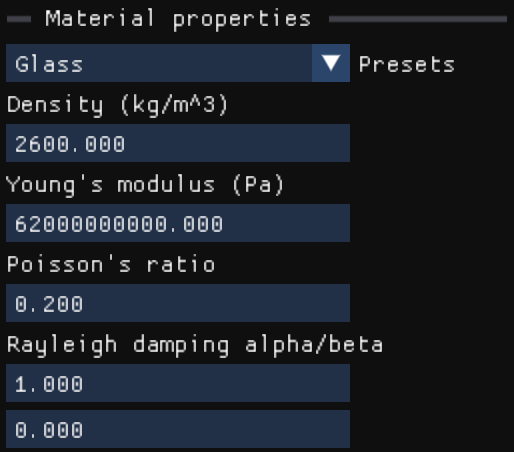
\includegraphics[width=0.5\linewidth]{images/MaterialProperties.png}
  \caption{Application UI section for material property configuration}
  \label{fig:MaterialProperties}
\end{figure}

After computing the mass and stifness matrices, the system's eigenvalues and eigenvectors are estimated using the Spectra C++ library \cite{spectra} to solve the elastodynamic eigenvalue problem (\ref{eq:EigenvalueProblem}) (using \verb|SymGEigsShiftSolver| method, providing the lowest expected frequency of 20 Hz as the shift $\sigma$ value).

Finally we compute the mode parameters from the estimated eigenvalues and eigenvectors (which are viewable in the UI for debugging purposes \ref{fig:ModeDebugUI}).

\begin{figure}
  \centering
  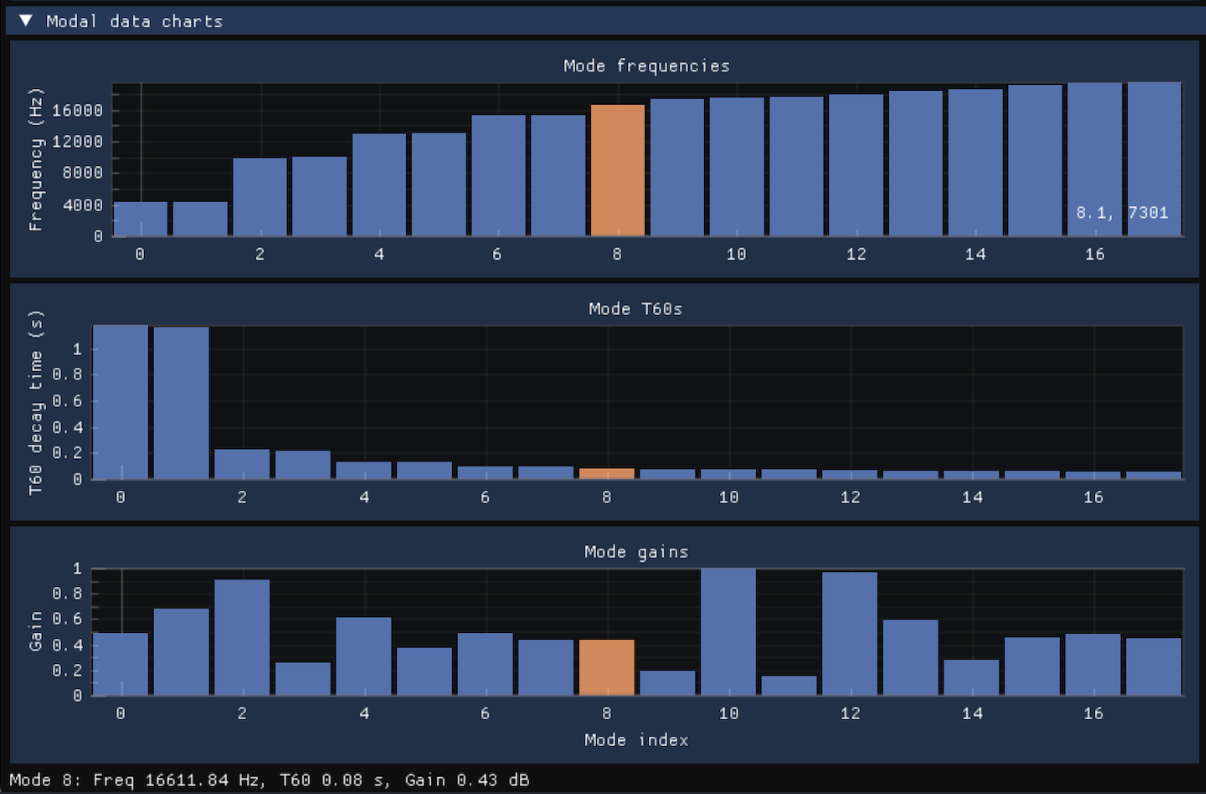
\includegraphics[width=0.5\linewidth]{images/ModalDebugUI.png}
  \caption{Application UI section for viewing all estimated modal parameters}
  \label{fig:ModeDebugUI}
\end{figure}

\subsection{Integration (Audio Rendering)}

As explained in the LMA section above, each resonating mode is modelled as an exponentially decaying sinusoid with an independent frequency, gain, and resonance duration.
Rather than implementing them as sine waves with exponential envelopes, using resonant bandpass filters allows any signal to excite the vertices (modes).
Mode filters are implemented as a parallel bank of biquad filters (Fig. 1), each with transfer function (Fig. 2)
\begin{equation}\label{eq:1}
H(z) = g\frac{1-z^{-2}}{1+\alpha_1z^{-1}+\alpha_2z^{-2}},
\end{equation}
with $\alpha_1 = -2\tau \cos\omega ,\ \alpha_2 = \tau^2,\ \omega = \frac{2\pi f}{f_s},$ and $\tau = 0.001^{\frac{1}{t_{60}}}.$
Here, $g$ is the mode gain, $f$ the mode frequency in Hz, $f_s$ is the sampling rate (always 48 kHz in this study), and $t_{60}$ is the \textit{T60 decay time} - the time it takes for the mode to decay by 60 dB from its initial amplitude.

Referring back to the \textit{LMA} section above, the mode frequencies correspond to the eigenvalues (and the damping factor), the gains are determined from the eigenvectors and the excitation force, and the T60 values are derived from the mode damping factors.

The full audio pipeline is implemented with a generated Faust Faust (Functional Audio Stream) programming language \cite{faust} DSP program.
Faust compiles the audio graph described in the DSP code to LLVM instructions (using LLVM JIT compilation), and executes the compiled graph sample-by-sample in real-time.
Generated audio buffers are streamed to the native audio device using the miniaudio C library \cite{miniaudio}.

Shown below are components of the signal-flow block diagram produced by the \verb|faust2svg| command from one such generated DSP program.
The top-level signal-flow diagram (\ref{fig:FaustProcess}) shows the impact "hammer" model component feeding into the modal model component.

The hammer is a simple model composed of a short pulse of white noise windowed by an attack-release envelope and smoothed by a lowpass filter, with "hardness" corresponding to pulse width and "size" corresponding to lowpass cutoff wavelength.
\footnote{This is an adaptation of a method for piano hammer modeling used in \href{https://ccrma.stanford.edu/~jos/pasp/Commuted_Piano_Synthesis.html}{commuted synthesis} \cite{smith_pasp}.
Despite its simplicity, the method has physical justification, but here is best regarded as a short injection of wideband energy at a mesh vertex, used to excite all modes.}
The hammer model is described by the following Faust expression (shown below in Figure \ref{fig:FaustHammer}):

\newpage

\begin{small}
\begin{verbatim}
hammer(trig, hardness, size) = en.ar(att, att, trig) * no.noise :
  fi.lowpass(3, ctoff) with {
    ctoff = (1-size)*9500 + 500;
    att = (1-hardness)*0.01 + 0.001;
  };
\end{verbatim}
\end{small}

Figure \ref{fig:FaustModeDiagrams} below shows the signal-flow diagram of the biquad filter bank, along with a detailed view of a single mode filter implementing the difference equation for the transfter function \hyperref[eq:1]{H(z)} above.

\begin{figure}
  \centering
  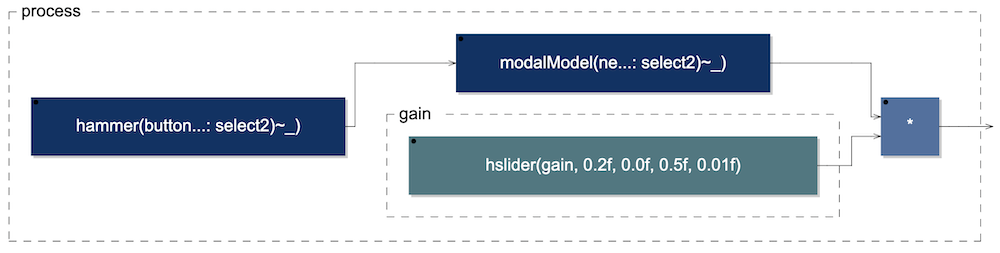
\includegraphics[width=\linewidth]{images/FaustProcess.png}
  \caption{Top-level Faust signal-flow diagram showing a hammer model exciting a modal model}
  \label{fig:FaustProcess}
\end{figure}
\begin{figure}
  \centering
  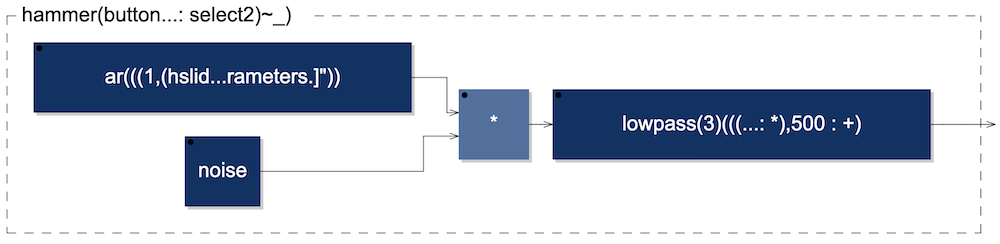
\includegraphics[width=\linewidth]{images/FaustHammer.png}
  \caption{Signal-flow diagram of the hammer model}
  \label{fig:FaustHammer}
\end{figure}
\begin{figure}
  \centering
  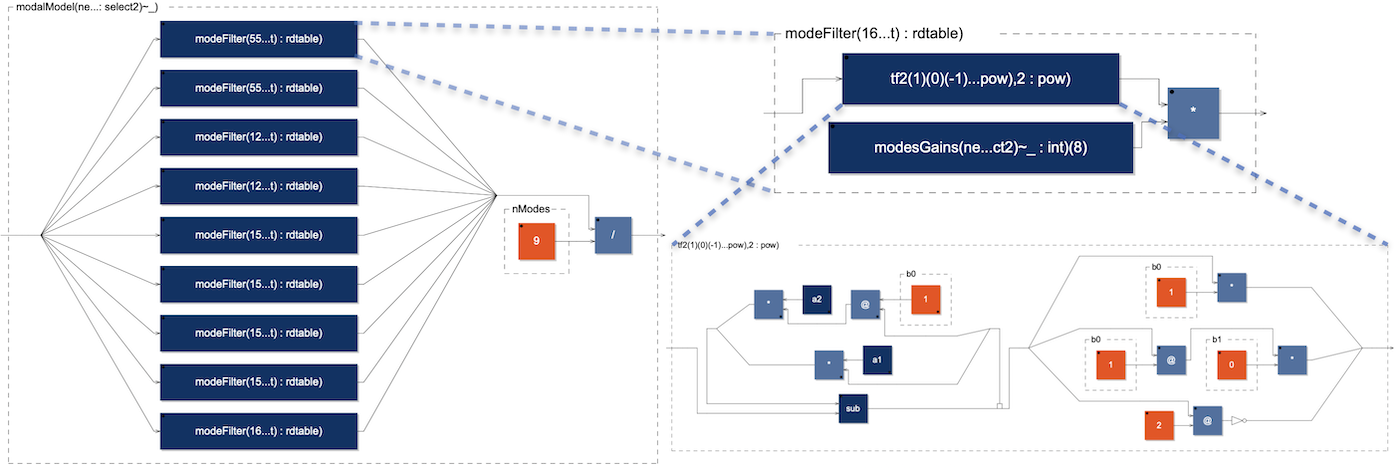
\includegraphics[width=\linewidth]{images/FaustModeDiagrams.png}
  \caption{Signal-flow diagram of the modal model. \textit{Left:} Parallel bank of mode biquad filters. \textit{Right:} Single mode filter implementing $H(z)$}
  \label{fig:FaustModeDiagrams}
\end{figure}

A full example generated Faust DSP program is provided in the appendix \ref{sec:FaustCode}.

\section{Results}

While implementing the prior \textit{Mesh2Audio} work (which focused on modeling bells), we were frustrated that, while the results \textit{sounded} reasonably realistic, we had no way to evaluate the accuracy of the rendered audio.
One of the main aspirations of this project was to address this issue.
\textit{RealImpact} was published shortly after completion of \textit{Mesh2Audio}, introducing a generous dataset tailored to address exactly this derth of publicly available data.
Producing such a dataset is challenging and resource intensive, and (to the knowledge of the authors) no dataset approaches its quality and quantity.
It has been immensely valuable to have side-by-side comparisons available.
However, in this project we were unable to find robust methods or metrics for quantitative evaluation, as we had originally hoped.

An ideal evaluation metric would closely match subjective judgement of audio similarity.
Many perceptual audio loss functions \cite{elbaz_perceptual_2017} and perceptually-motivated signal transforms \cite{smith_bark_1999} have been proposed, offering direct comparison of time or frequency-domain audio signals.
However, given the specific context of modal audio synthesis, in which the entire signal is a superposition of pure sinuoid modes with known frequency, I wanted to take advantage of this known low-dimensional latent representation.
There are \href{https://ccrma.stanford.edu/~jos/pasp/Modal_Expansion.html}{several known methods} \cite{smith_pasp} for estimating the resonant mode frequencies, gains, and decay times directly from spectra.
If successfully applied, this would offer direct comparison of all estimated modal parameters with their estimated counterparts in the target real-world recorded impacts.
However, these methods are complex and often unreliable.
As a preliminary step, we investigated simply comparing the $M$ estimated mode frequencies (ignoring the gains and decay times) with the top-$M$ peak frequencies in the real-world impact spectra.
However, we encountered several difficulties using even this simple approach:
\begin{itemize}
  \item Many \textit{RealImpact} recordings have a low signal-to-noise ratio, causing spurious false frequency maxima uncorrelated with the resonant modes.
  \item We observed it is very common for modal analysis to find modes in pairs with closely-spaced frequencies \textit{degenerate modes} \cite{afolabi_degenerate_modes} (see \ref{fig:DegenerateModePairs}).
  \item Degenerate modes pose one difficulty in matching frequencies between the generated and target spectra, but frequency-matching is a nontrivial problem, since the number of true modes is unknown, and it's not generally possible to distinguish between incorrect, missing, or spurious modes.
  \item Even a perfect model is only as accurate as its inputs. Generic material properties (\ref{tab:MaterialProperties}) may differ significantly from those of the real household objects, and the 3D scans may be missing important geometry.
  \item Finally, the impact recordings are affected by the recording environment and acoustic dynamics, while our modal model "records" a direct signal from the object's surface vibrations, making comparisons difficult even with a perfect model and input data.
\end{itemize}

\begin{figure}
  \centering
  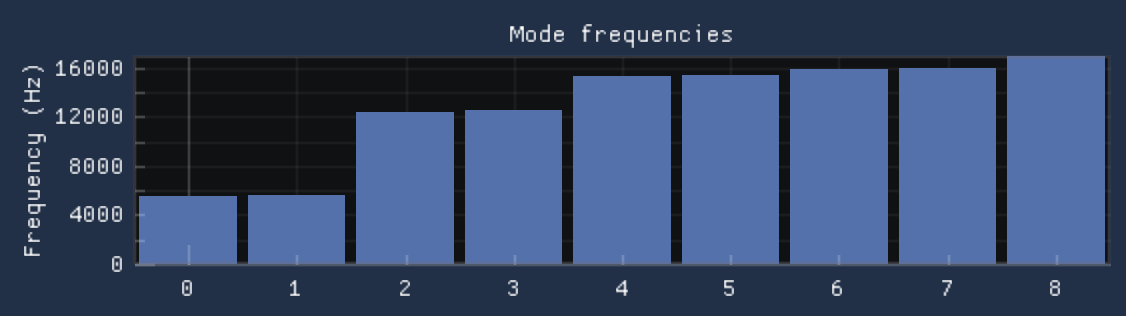
\includegraphics[width=\linewidth]{images/DegenerateModePairs.png}
  \caption{An example of estimated mode frequencies occuring in closely-spaced frequency pairs (\textit{degenerate pairs})}
  \label{fig:DegenerateModePairs}
\end{figure}

Due to these challenges, we found that e.g. a straightforward RMSE of spectral peaks, was not only inaccurate in the absolute sense, but was not even reliable for relative comparisons.
Thus, the results we present here are mostly qualitative.

\subsection{Subjective evaluation}

Subjectively, the most important perceptual factor is the fundamental frequency.
We observed that for almost all \textit{RealImpact} objects, the raw FEM-estimated modal frequencies were shifted \textit{up} in frequency.
It could also be that low-freqency true modes are often simply not found.
However, since simply scaling frequencies often results in reasonably close mappings to true modes in the low-frequency range, we believe the most likely explanation for this failure mode is inaccurate material parameters.

To remedy this issue, when generating a modal model for which a true recording is present, we scale all mode frequencies to set the lowest mode equal to the peak frequency in the true spectrum.
This naive approach is not always accurate, but it addresses the majority of mismatches.

Another common failure mode is underestimating damping.
The model, as implemented, seems to have a strong bias for resonating much longer than real-world objects, across modes.
The mismatch is not extreme or consistent enough to strongly indicate a fundamental error in calculation or scaling, although it is certainly possible.

\subsection{Quantitative and qualitative evaluation}

The table below shows spectrum comparisons between synthesized and real-world recorded spectra \ref{tab:SpectrumComparison} in response to "striking" various meshes at the same position (rounded to the resolution of the 3D-scanned meshes).
The cylinders shown in the images represent recorded microphone positions, but all real-world spectra shown are from recorded from a single microphone centered near the impacted object, and the modal audio model does not implement any audio wave radiation modeling.
(Again, all modal audio samples are generated by extracting estimated surface vibrations, as if recorded from a contact microphone.)

The spectra are measured from 30 frames to 3,000 frames (1/16 of a second) after impact.
The 30-frame start buffer provides a short time for nonlinear contributions to decay, and the duration is long enough to accurately resolve modes as low as 32 Hz (well below the expected fundamental vibrational mode of these small household objects).
A Blackman–Harris window is applied to the audio signal before applying the FFT.

It is clear from brief examination of the spectra that the synthesized results are far from quantitatively accurate reconstructions of the target impact responses.
Much of the discrepency is due to high noise levels in the real-world recordings (while the synthesized results, are composed of pure sinusoidal components).
But there are clearly prominent and perceptually relevant resonant modes that are unaccounted for in the synthesized audio.

The README of the \href{https://github.com/khiner/MeshEditor}{project GitHub repo} contains links to the corresponding audio samples.
Although the synthesized samples are by no means perceptually identical to the real-world recordings, I find many to be surprisingly close, given all the inherent issues outlined above.

\begin{table}[!ht]
  \centering
  \caption{Comparison of Mesh, Modal Spectrum, and Real Spectrum for Various Objects}
  \label{tab:SpectrumComparison}
  \begin{tabular}{|c|c|c|}
  \hline
  \textbf{Object Name} & \textbf{Mesh} & \textbf{Synthesized/Real Spectra} \\ \hline
  Ceramic Koi Bowl & 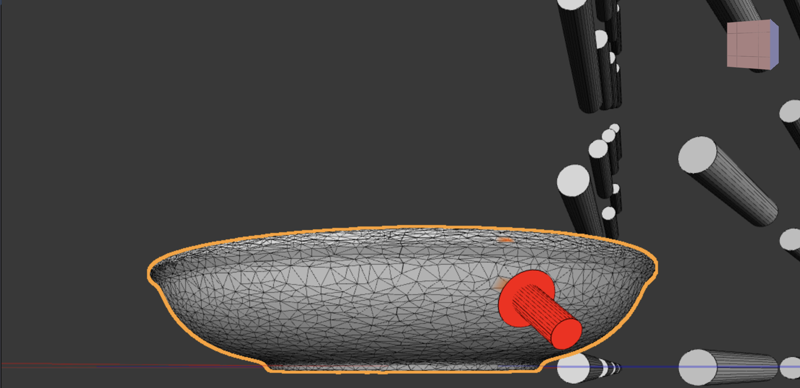
\includegraphics[width=0.2\textwidth]{images/impacts/CeramicKoiBowlMesh.png} & 
  \begin{subfigure}{0.3\linewidth}
    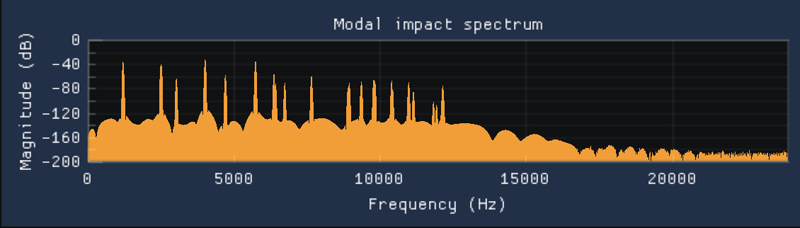
\includegraphics[width=\linewidth]{images/impacts/CeramicKoiBowlModal.png}
    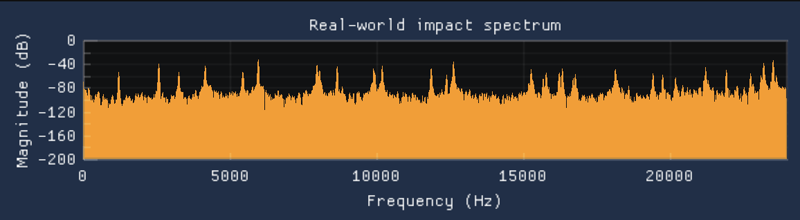
\includegraphics[width=\linewidth]{images/impacts/CeramicKoiBowlReal.png}
  \end{subfigure} \\ \hline
  Ceramic Pitcher & 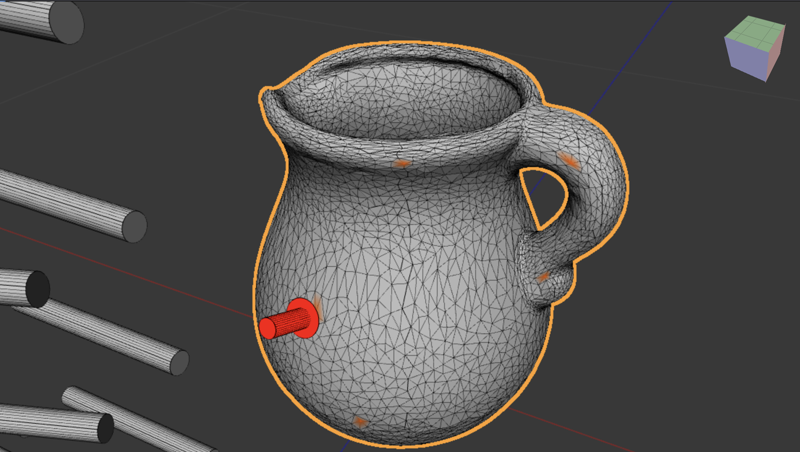
\includegraphics[width=0.2\textwidth]{images/impacts/CeramicPitcherMesh.png} & 
  \begin{subfigure}{0.3\linewidth}
    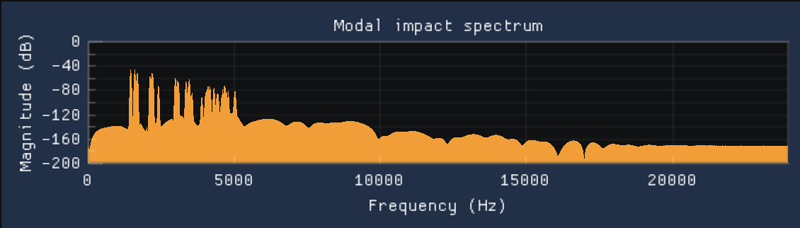
\includegraphics[width=\linewidth]{images/impacts/CeramicPitcherModal.png}
    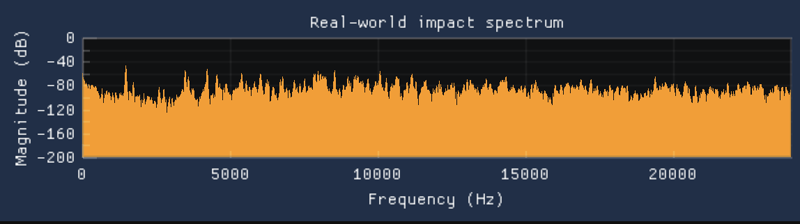
\includegraphics[width=\linewidth]{images/impacts/CeramicPitcherReal.png}
  \end{subfigure} \\ \hline
  Glass Cup & 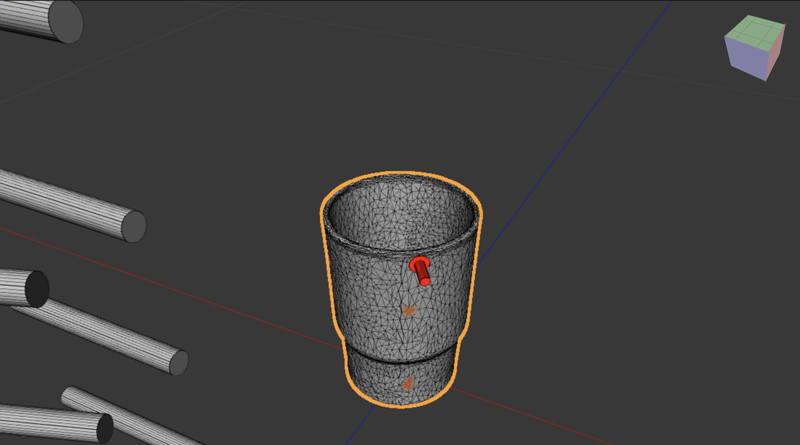
\includegraphics[width=0.2\textwidth]{images/impacts/GlassCupMesh.png} & 
  \begin{subfigure}{0.3\linewidth}
    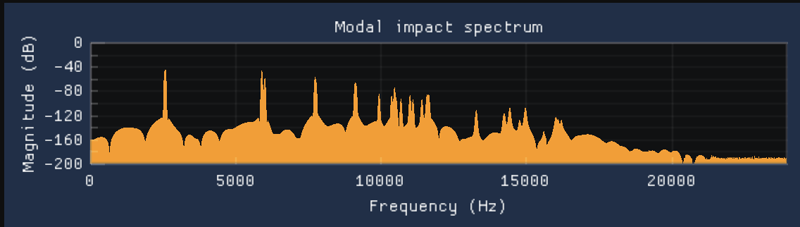
\includegraphics[width=\linewidth]{images/impacts/GlassCupModal.png}
    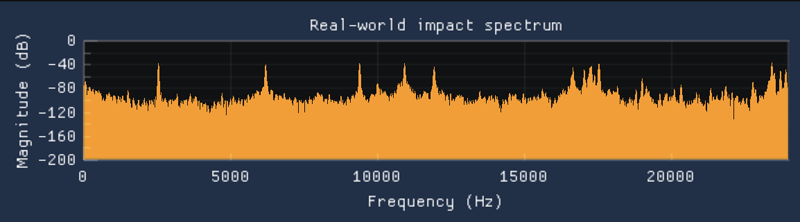
\includegraphics[width=\linewidth]{images/impacts/GlassCupReal.png}
  \end{subfigure} \\ \hline
  Iron Mortar & 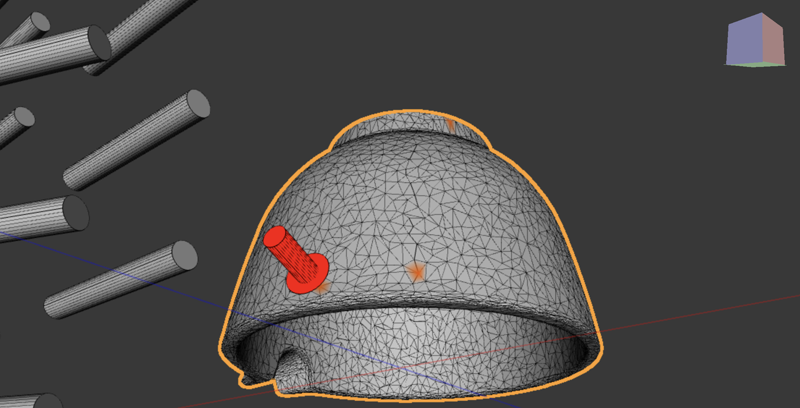
\includegraphics[width=0.2\textwidth]{images/impacts/IronMortarMesh.png} & 
  \begin{subfigure}{0.3\linewidth}
    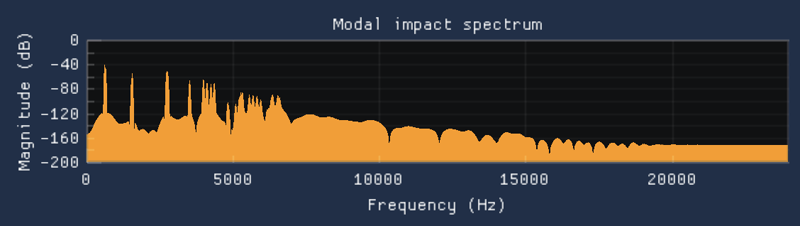
\includegraphics[width=\linewidth]{images/impacts/IronMortarModal.png}
    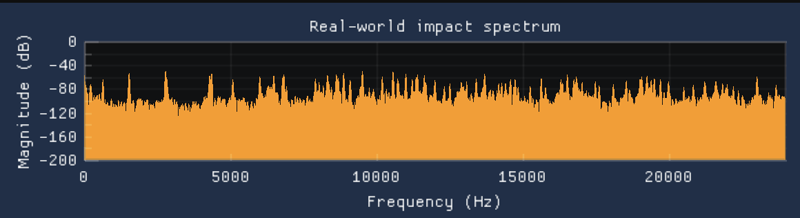
\includegraphics[width=\linewidth]{images/impacts/IronMortarReal.png}
  \end{subfigure} \\ \hline
  Iron Skillet & 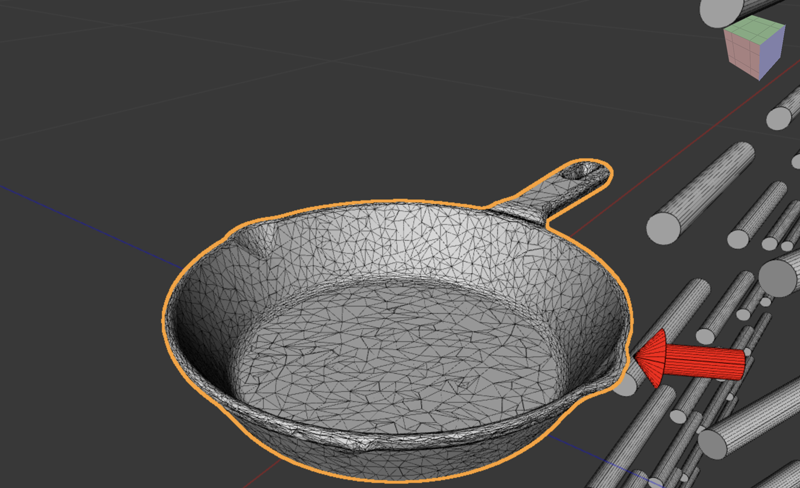
\includegraphics[width=0.2\textwidth]{images/impacts/IronSkilletMesh.png} & 
  \begin{subfigure}{0.3\linewidth}
    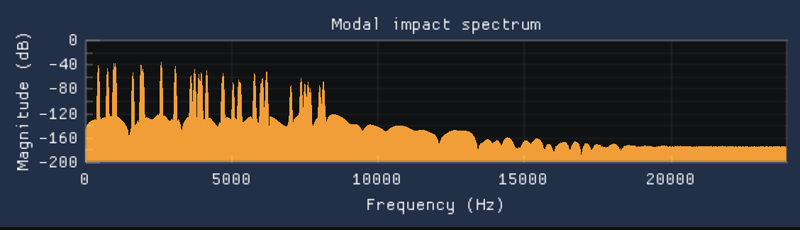
\includegraphics[width=\linewidth]{images/impacts/IronSkilletModal.png}
    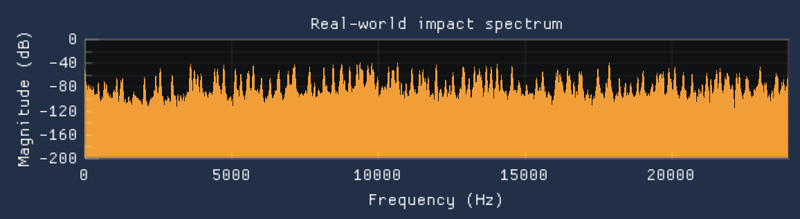
\includegraphics[width=\linewidth]{images/impacts/IronSkilletReal.png}
  \end{subfigure} \\ \hline
  Plastic Scoop & 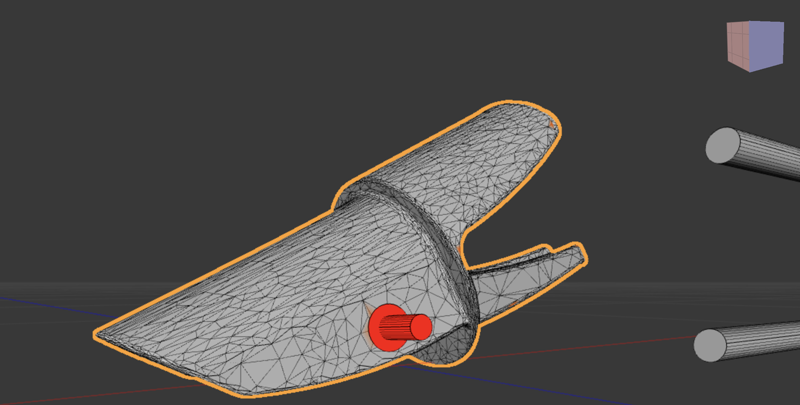
\includegraphics[width=0.2\textwidth]{images/impacts/PlasticScoopMesh.png} & 
  \begin{subfigure}{0.3\linewidth}
    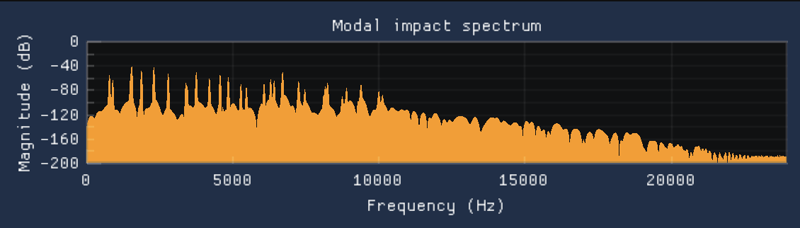
\includegraphics[width=\linewidth]{images/impacts/PlasticScoopModal.png}
    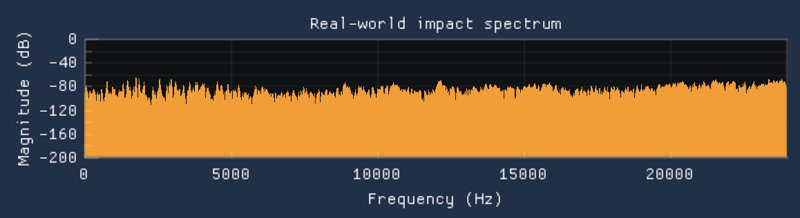
\includegraphics[width=\linewidth]{images/impacts/PlasticScoopReal.png}
  \end{subfigure} \\ \hline
  Swan Small Ceramic & 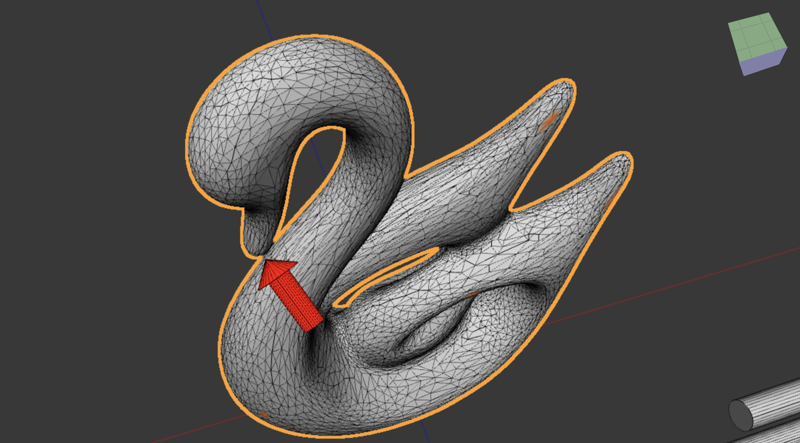
\includegraphics[width=0.2\textwidth]{images/impacts/SwanSmallCeramicMesh.png} & 
  \begin{subfigure}{0.3\linewidth}
    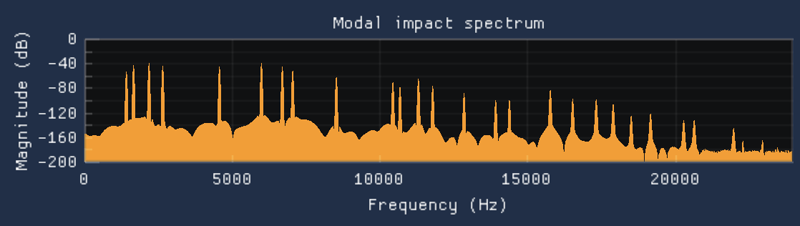
\includegraphics[width=\linewidth]{images/impacts/SwanSmallCeramicModal.png}
    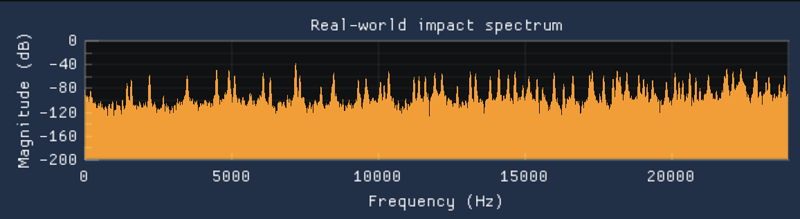
\includegraphics[width=\linewidth]{images/impacts/SwanSmallCeramicReal.png}
  \end{subfigure} \\ \hline
  \end{tabular}
\end{table}

\section{Summary and conclusions}

Overall, these results show that Linear Modal Analysis/Synthesis is an effective and highly efficient method for physically plausible audio synthesis of rigid body.

In addition to the many issues outlined above, the linear assumption has perceptible impact on physical accuracy, especially few modes are estimated.

These experiments seem to indicate that it is possible to acheive an overall impression of perceived audio similarity while failing to achieve close alignment in spectral composition.
This is testament to the perceptual importance of non-spectral aspects such as fundamental frequency and dynamic envelope, and underlines the crucial importance of developing suitable datasets.
As immersive environments such as augmented and virtual realities become increasingly capable and visual rendering fidelity improves, rigourous testing of simulated acoustics against real-world will become increasingly important to ensure that acoustic realism keeps pace.

Continuing to develop real-world audio datasets alongside model improvements will also provide opportunities for data-driven audio generation models, for example by nudging fully differentiable physically-informed models \cite{engel_ddsp_2019} \cite{wang_neural_2019} towards natural audio manifolds.

\bibliographystyle{plain}
\bibliography{bibliography}

\newpage

\appendix

\section{Complete model Faust code}
\label{sec:FaustCode}
The following is a complete example Faust DSP code output, including the full modal model and parameter UI specification, excluding only tooltip help text.
\verb|mode...| floading point values are condensed with ellipses for brevity.

\begin{small}
\begin{verbatim}
import("stdfaust.lib");

modalModel(freq,exPos,t60Scale) = _ <: par(
  mode,nModes,
  pm.modeFilter(modeFreqs(mode),modesT60s(mode),modesGains(int(exPos),mode))
) :> /(nModes)
with{
  nModes = 30;
  nExPos = 5;
  modeFreqRatios(n) = ba.take(n+1,(1,1.01168,2.25071,...));
  modeFreqs(mode) = freq*modeFreqRatios(mode);
  modesGains(p,n) = waveform{0.435705,0.726901,0.825358,...},
                    int(p*nModes+n) :
                    rdtable : select2(modeFreqs(n)<(ma.SR/2-1),0);
  modesT60s(n) = t60Scale * ba.take(n+1,(0.717945,0.701597,0.142672,...));
};
gate = button("Gate");
hammerHardness = hslider("Hammer hardness",0.9,0,1,0.01) : ba.sAndH(gate);
hammerSize = hslider("Hammer size",0.1,0,1,0.01) : ba.sAndH(gate);
gain = hslider("Gain[scale:log]",0.2,0,0.5,0.01);
freq = hslider("Frequency[scale:log]",2569,60,26000,1) : ba.sAndH(gate);
exPos = nentry("Excite index",2,0,4,1) : ba.sAndH(gate);
t60Scale = hslider("t60[scale:log]",1,0.1,10,0.01) : ba.sAndH(gate);
 
hammer(trig,hardness,size) = en.ar(att,att,trig)*no.noise :
  fi.lowpass(3,ctoff)
with{ ctoff = (1-size)*9500+500; att = (1-hardness)*0.01+0.001; };
 
process = hammer(gate,hammerHardness,hammerSize) :
  modalModel(freq,exPos,t60Scale)*gain;
\end{verbatim}
\end{small}

\end{document}
